% ============================================================
%  CHAPTER 4: SYSTEM ARCHITECTURE AND DESIGN
% ============================================================

\chapter{SYSTEM ARCHITECTURE AND DESIGN}
\label{chap:system_design}

\section{Overall Architectural Philosophy and Multi-Tier Topology}
\label{sec:overall_architecture_philosophy}

The QuantumSafe VPN system is architected as an end-to-end, multi-tier secure tunneling framework designed to provide unconditional post-quantum forward secrecy for mobile endpoints traversing untrusted public networks. The architecture adheres to four foundational design principles:

\begin{enumerate}
    \item \textbf{Separation of Concerns}: The system decouples the user interface, reactive state management, background OS service execution, cryptographic wire operations, and kernel packet I/O into distinct, loosely coupled modular layers.
    \item \textbf{Zero-Trust Transit Boundary}: The intermediate transport network (Wi-Fi, cellular, ISP routing) is treated as completely hostile. No cleartext metadata, session tokens, or unauthenticated packet framing may traverse this boundary under any circumstance.
    \item \textbf{Kernel-Enforced Isolation}: The architecture leverages operating system kernel facilities---\texttt{android.net.VpnService} with \texttt{protect()} on Android, and the Linux Universal TUN/TAP driver with \texttt{iptables} NAT masquerading on the server---to guarantee that packet interception and routing loop prevention are enforced deterministically at the kernel boundary rather than via fragile user-space workarounds.
    \item \textbf{Strict Post-Quantum Cryptographic Opinionation}: Rather than implementing dynamic, runtime-negotiated cipher suites (which introduce downgrade attack vectors such as SSL/TLS stripping), the wire protocol enforces a fixed, hardened post-quantum cipher suite: ML-KEM-1024 for key agreement, ML-DSA-65 for authentication, HKDF-SHA256 for key derivation, and AES-256-GCM for packet encapsulation.
\end{enumerate}

Figure~\ref{fig:deployment_topology_arch} illustrates the high-level network deployment topology connecting the mobile client tier, intermediate wireless networks, the Linux gateway, and upstream Internet destinations.

\begin{figure}[htbp]
  \centering
  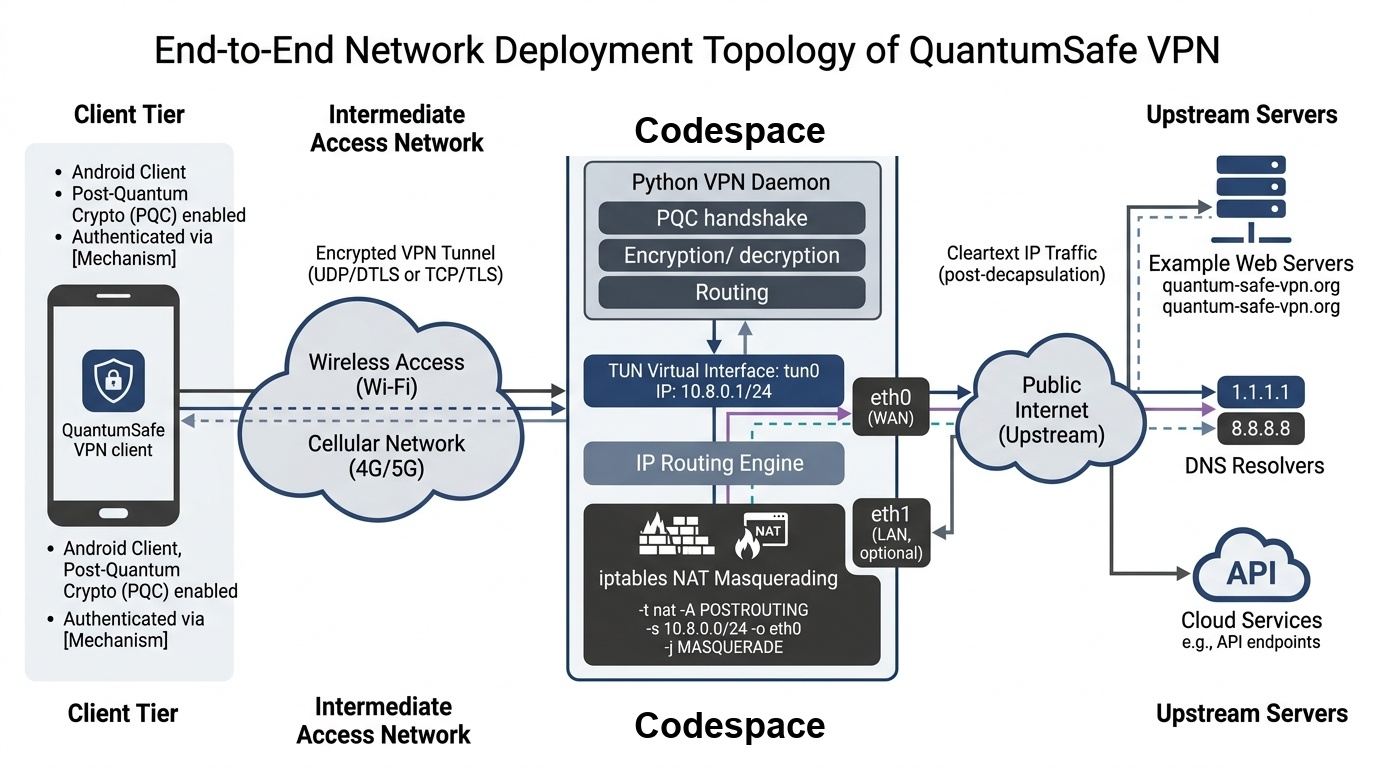
\includegraphics[width=0.92\linewidth,height=0.45\textheight,keepaspectratio]{figures/deployment_topology_concept.jpg}
  \caption{End-to-End Network Deployment Topology of QuantumSafe VPN.}
  \label{fig:deployment_topology_arch}
\end{figure}

\section{Comparison of Legacy vs. Proposed Architecture}
\label{sec:legacy_vs_proposed_arch}

To establish the technical evolution of the system, Table~\ref{tab:legacy_vs_proposed_comparison} details the comparative architectural shift from the preliminary laboratory Python prototype to the production Android-to-Linux enterprise architecture.

\begin{table}[htbp]
  \centering
  \small
  \caption{Architectural Comparison: Legacy Python Desktop vs. Proposed Native Android System.}
  \label{tab:legacy_vs_proposed_comparison}
  \begin{tabular}{@{}P{3.2cm}P{5.2cm}P{5.8cm}@{}}
    \toprule
    \textbf{Dimension} & \textbf{Legacy Desktop System} & \textbf{Proposed Android System} \\
    \midrule
    \textbf{Client Platform} & Linux Desktop / CLI & Android Mobile (API 26--34) \\
    \textbf{UI Architecture} & None (stdout terminal output) & Reactive Jetpack Compose (Material 3 Minimal White) \\
    \textbf{Process Model} & Synchronous blocking Python script & Asynchronous Kotlin Coroutines with \texttt{StateFlow} \\
    \textbf{TUN Management} & Direct \texttt{/dev/net/tun} (Root required) & Sandboxed \texttt{android.net.VpnService} (User consented) \\
    \textbf{Loop Prevention} & Shell script \texttt{ip rule} routing & Kernel socket tagging via \texttt{protect(socket)} \\
    \textbf{Crypto Engine} & CPython bindings to \texttt{liboqs} & Pure-Kotlin lattice engine with SHA3-256 alignment \\
    \textbf{Session Persistence} & Volatile in-memory variables & Android Keystore backed \texttt{SecurityManager} \\
    \textbf{Gateway Dispatch} & Single-client prototype & Multi-client dynamic IP allocation (\texttt{ip\_pool.py}) \\
    \bottomrule
  \end{tabular}
\end{table}

\section{Proposed Native Android Architectural Layers}
\label{sec:android_layered_architecture}

The Android mobile client is organized into five cohesive architectural layers following the Model-View-ViewModel (MVVM) software architectural pattern:

\begin{enumerate}
    \item \textbf{Presentation Layer (Jetpack Compose UI)}: Renders the minimal white-theme user interface using declarative composable functions (\texttt{MainScreen}, \texttt{HomeScreen}, \texttt{ServerConfigScreen}, \texttt{SecurityDetailsScreen}, \texttt{SettingsScreen}). It observes immutable state flows emitted by the ViewModel and dispatches user actions without directly accessing system networking or cryptographic APIs.
    \item \textbf{ViewModel Layer (\texttt{VpnViewModel})}: Acts as the architectural bridge between the UI and background services. It manages application state (\texttt{VpnState}, telemetry counters, configuration models) using Kotlin Coroutines and reactive \texttt{StateFlow} observables, surviving Android configuration changes (such as screen rotations).
    \item \textbf{Inter-Process Communication Bridge (\texttt{VpnServiceBridge})}: Maintains thread-safe, decoupled event communication between the UI/ViewModel and the background \texttt{VpnService}. It coordinates service binding, command dispatching (Connect, Disconnect), and real-time telemetry streaming via high-throughput \texttt{SharedFlow} channels.
    \item \textbf{Service and Network Layer (\texttt{QuantumSafeVpnService})}: Extends Android's \texttt{android.net.VpnService}. It executes as an Android Foreground Service, manages the virtual TUN interface lifecycle via \texttt{ParcelFileDescriptor}, enforces socket protection via \texttt{protect()}, and runs dedicated asynchronous coroutines for bidirectional packet forwarding.
    \item \textbf{Cryptographic Wire Engine (\texttt{PqcEngine})}: A specialized, pure-Kotlin cryptographic library executing ML-KEM-1024 key encapsulation, ML-DSA-65 signature verification, pure-Kotlin Keccak-$f[1600]$ SHA3-256 hashing, HKDF-SHA256 session key expansion, and AES-256-GCM line-rate authenticated packet encryption.
    \item \textbf{Secure Storage Layer (\texttt{SecurityManager})}: Encapsulates Android Keystore operations, persisting server hostnames, port numbers, custom MTUs, and server identity pinning fingerprints within hardware-encrypted shared preferences.
\end{enumerate}

\section{Client-Server Interaction Model and Connection Lifecycle}
\label{sec:client_server_lifecycle}

The operational interaction between the Android mobile client and the Linux VPN gateway transitions through six well-defined operational phases:

\begin{enumerate}
    \item \textbf{Phase 1: Initialization and Authorization}: The user requests connection initiation. The Android application invokes \texttt{VpnService.prepare()}. If authorized by the user, the application spins up \texttt{QuantumSafeVpnService} with a persistent foreground notification, establishing an active \texttt{CONNECTING} state.
    \item \textbf{Phase 2: Socket Bypassing and Transport Setup}: The service establishes a non-blocking TCP socket to the gateway's public IP address on port 7000. Prior to initiating the TCP handshake, the service invokes \texttt{protect(socket)}, commanding the Linux kernel that all traffic emitted by this socket must bypass the virtual VPN interface.
    \item \textbf{Phase 3: 4-Stage Post-Quantum Handshake}: The client and server execute the synchronized cryptographic exchange over the protected TCP stream:
    \begin{itemize}
        \item \textit{Stage 1}: Server sends its persistent ML-DSA-65 public key (1,952 bytes). Client verifies the public key against pinned identity hashes.
        \item \textit{Stage 2}: Client generates an ephemeral ML-KEM-1024 keypair and transmits its public key (1,568 bytes) to the server.
        \item \textit{Stage 3}: Server encapsulates a 32-byte shared secret under the client's public key, signs the complete handshake transcript using ML-DSA-65, and transmits the 1,568-byte ciphertext and 3,309-byte signature alongside the client configuration JSON payload.
        \item \textit{Stage 4}: Client verifies the ML-DSA-65 signature, decapsulates the shared secret using its ML-KEM-1024 secret key, and both endpoints derive identical 256-bit AES-GCM session keys via HKDF-SHA256.
    \end{itemize}
    \item \textbf{Phase 4: Virtual TUN Interface Construction}: The client parses the configuration JSON payload, extracting the assigned client IP (e.g., \texttt{10.8.0.2}), virtual netmask (\texttt{255.255.255.0}), gateway DNS servers (\texttt{1.1.1.1}, \texttt{8.8.8.8}), and MTU (\texttt{1400}). The \texttt{VpnService.Builder} instantiates the TUN interface, returning a valid \texttt{ParcelFileDescriptor}. The UI transitions to \texttt{CONNECTED}.
    \item \textbf{Phase 5: Bidirectional Encrypted Tunneling}: Two concurrent background worker loops execute:
    \begin{itemize}
        \item \textit{Uplink Loop}: Reads outbound raw IPv4 datagrams from TUN, prepends a monotonic 64-bit sequence counter, encrypts via AES-256-GCM, prefixes with 4-byte big-endian framing, and writes to the TCP socket.
        \item \textit{Downlink Loop}: Reads frames from TCP socket, authenticates 16-byte GCM tags, validates sequence counters against replay attacks, decrypts payloads, and writes raw IPv4 packets into the TUN interface.
    \end{itemize}
    \item \textbf{Phase 6: Graceful Teardown}: Upon user disconnection, error detection, or network loss, the service flushes packet buffers, transmits an optional teardown frame, closes socket channels, releases the file descriptor, dismisses the foreground notification, and transitions to \texttt{DISCONNECTED}.
\end{enumerate}

\section{Android \texttt{VpnService} Integration and Socket Protection}
\label{sec:vpn_service_integration_protect}

The architectural linchpin of the mobile client is the seamless integration of Android's \texttt{VpnService}. When the application configures the virtual interface:
\begin{lstlisting}[language=Kotlin, caption={Virtual TUN Interface Configuration in QuantumSafeVpnService.}]
val builder = Builder()
    .setSession("QuantumSafe VPN")
    .setMtu(mtu)
    .addAddress(assignedClientIp, 24)
    .addRoute("0.0.0.0", 0) // Capture all IPv4 traffic
    .addDnsServer("1.1.1.1")
    .addDnsServer("8.8.8.8")
    .setBlocking(true)

vpnInterface = builder.establish()
\end{lstlisting}

Setting \texttt{addRoute("0.0.0.0", 0)} updates the Linux kernel policy routing table, establishing the TUN device as the default gateway for all UID traffic. However, to prevent the catastrophic recursive routing loop explained in Section~\ref{sec:mobile_network_challenges}, the TCP socket connecting to the server gateway is explicitly shielded:

\begin{lstlisting}[language=Kotlin, caption={Kernel-Level Socket Protection via protect().}]
val socketChannel = SocketChannel.open()
socketChannel.configureBlocking(true)

// Explicitly protect socket from VPN routing table
val protected = protect(socketChannel.socket())
if (!protected) {
    throw IllegalStateException("Failed to protect VPN transport socket!")
}

// Connect to remote gateway after protection is verified
socketChannel.connect(InetSocketAddress(serverHost, serverPort))
\end{lstlisting}

Under the hood, \texttt{protect()} invokes a native C-library system call in AOSP's \texttt{libandroid\_runtime.so}, executing \texttt{setsockopt(fd, SOL\_SOCKET, SO\_MARK, ...)} to mark outgoing socket buffers with a dedicated routing tag (\texttt{0xf0000} or equivalent vendor tag). The Linux kernel routing policy engine (\texttt{ip rule}) evaluates this mark and routes the packet through the physical underlying network table (\texttt{wlan0} or cellular) rather than the default \texttt{0.0.0.0/0} TUN rule.

\section{Linux Gateway TUN Interface and IP Routing Architecture}
\label{sec:linux_gateway_routing_arch}

On the server side, the companion Python daemon (\texttt{vpn/tunnel\_server.py}) interacts directly with the Linux kernel's Universal TUN/TAP driver (\texttt{tun0}). The server's networking architecture comprises three cooperating modules:

\begin{enumerate}
    \item \textbf{Dynamic IP Pool Allocator (\texttt{vpn/ip\_pool.py})}: Manages a thread-safe pool of client virtual addresses within the \texttt{10.8.0.0/24} subnet (allocating \texttt{10.8.0.2} through \texttt{10.8.0.254}). It maps each connected client's physical socket endpoint to its assigned virtual IP.
    \item \textbf{Session Router (\texttt{SessionRouter})}: Maintains active client session records, mapping each assigned virtual IP to its corresponding TCP socket, negotiated AES-256-GCM session key, and independent send/receive sequence counters.
    \item \textbf{NAT Forwarding and Masquerading Manager (\texttt{vpn/nat\_manager.py})}: Automates Linux kernel IP packet forwarding by setting \texttt{sysctl net.ipv4.ip\_forward=1} and configuring \texttt{iptables} rules:
    \begin{lstlisting}[language=bash, caption={Linux Kernel NAT Masquerade Configuration.}]
iptables -t nat -A POSTROUTING -s 10.8.0.0/24 -o eth0 -j MASQUERADE
iptables -A FORWARD -i tun0 -o eth0 -j ACCEPT
iptables -A FORWARD -i eth0 -o tun0 -m state --state RELATED,ESTABLISHED -j ACCEPT
    \end{lstlisting}
\end{enumerate}

When an encrypted packet arrives from an Android client over TCP port 7000, the server decrypts the frame, extracts the inner IPv4 packet, and writes it directly to \texttt{tun0}. The Linux kernel inspects the packet's destination IP (e.g., a public web server), applies \texttt{iptables} NAT masquerading (substituting the client's \texttt{10.8.0.2} source IP with the server's public WAN IP), and routes it over the physical interface (\texttt{eth0}). When return packets arrive on \texttt{eth0}, the kernel de-masquerades the destination IP back to \texttt{10.8.0.2} and writes the packet to \texttt{tun0}. The server's \texttt{tun\_dispatcher\_loop} reads the packet from \texttt{tun0}, parses the destination IP (\texttt{10.8.0.2}), queries the \texttt{SessionRouter}, encrypts the packet with that client's unique AES session key, and transmits the frame back over TCP.

\section{Post-Quantum Wire Protocol Design and Binary Framing}
\label{sec:wire_protocol_framing}

To guarantee stream synchronization over TCP and protect against packet injection and fragmentation, QuantumSafe VPN implements a deterministic binary framing format across both handshake and data phases.

\subsection{Framing Prefix Structure}
Every transmission over the TCP stream begins with a mandatory 4-byte big-endian unsigned integer indicating the exact payload length:
\begin{equation}
\text{Header} = [\text{Length} : 4\text{ Bytes, Big-Endian uint32}] \parallel [\text{Payload} : \text{Length Bytes}]
\end{equation}
The receiver invokes an exact-byte reading loop (\texttt{recv\_exact}), ensuring that TCP stream chunking and packet coalescence do not desynchronize the application protocol stream.

\subsection{Handshake Message Schemas}
\begin{itemize}
    \item \textbf{Stage 1 (Server Hello)}:
    $$\text{Payload} = [\text{ML-DSA-65 Public Key} : 1,952\text{ Bytes}]$$
    \item \textbf{Stage 2 (Client Key Exchange)}:
    $$\text{Payload} = [\text{ML-KEM-1024 Ephemeral Public Key} : 1,568\text{ Bytes}]$$
    \item \textbf{Stage 3A (Server Ciphertext)}:
    $$\text{Payload} = [\text{ML-KEM-1024 Ciphertext} : 1,568\text{ Bytes}]$$
    \item \textbf{Stage 3B (Server Identity Signature)}:
    $$\text{Payload} = [\text{ML-DSA-65 Signature} : 3,309\text{ Bytes}]$$
    \item \textbf{Stage 3C (Client Configuration Block)}:
    $$\text{Payload} = \text{UTF-8 encoded JSON: } \{\text{"assigned\_ip"}, \text{"netmask"}, \text{"dns"}, \text{"mtu"}\}$$
\end{itemize}

\subsection{Data Tunnel Encapsulated Frame Structure}
During active VPN data transfer, every transmitted IP packet is encapsulated according to the binary wire structure depicted in Figure~\ref{fig:tikz_packet_framing}:
\begin{equation}
\label{eq:wire_framing_equation}
\text{Wire Frame} = \underbrace{[\text{Length} : 4\text{B}]}_{\text{Framing}} \parallel \underbrace{[IV : 12\text{B}]}_{\text{AES-GCM Nonce}} \parallel \underbrace{\text{AES-GCM}_{\text{Key}}\Big([\text{Seq} : 8\text{B}] \parallel [\text{Raw IPv4 Datagram}]\Big)}_{\text{Encrypted Payload}} \parallel \underbrace{[\text{Auth Tag} : 16\text{B}]}_{\text{Galois MAC}}
\end{equation}

\begin{figure}[htbp]
  \centering
  \begin{tikzpicture}[
    scale=0.88, every node/.style={transform shape},
    field/.style={draw=darkcharcoal, thick, fill=white, minimum height=1.2cm, align=center, font=\footnotesize\bfseries},
    headerfield/.style={field, fill=blue!10},
    ivfield/.style={field, fill=teal!10},
    seqfield/.style={field, fill=yellow!15},
    payloadfield/.style={field, fill=vpnblue!15},
    tagfield/.style={field, fill=red!10}
  ]
    % Outer Frame
    \node[headerfield, minimum width=2.4cm] (len) at (0, 0) {Frame Length\\(4 Bytes)};
    \node[ivfield, minimum width=2.4cm] (iv) at (2.4, 0) {GCM Nonce / IV\\(12 Bytes)};
    \node[seqfield, minimum width=2.6cm] (seq) at (4.9, 0) {Monotonic Seq\\(8 Bytes)};
    \node[payloadfield, minimum width=4.8cm] (data) at (8.6, 0) {Raw IPv4 Packet\\(Up to MTU Bytes)};
    \node[tagfield, minimum width=2.6cm] (tag) at (12.3, 0) {Auth Tag\\(16 Bytes)};

    % Brackets
    \draw[thick, decorate, decoration={brace, amplitude=6pt, mirror}] (-1.2, -0.9) -- (13.6, -0.9)
      node[midway, yshift=-0.5cm, font=\small\bfseries] {Total Wire Frame Transmitted over TCP Stream};

    \draw[thick, decorate, decoration={brace, amplitude=5pt}] (3.6, 0.9) -- (11.0, 0.9)
      node[midway, yshift=0.45cm, font=\footnotesize\bfseries, text=vpnblue] {Plaintext Authenticated \& Encrypted via AES-256-GCM};
  \end{tikzpicture}
  \caption{Binary Wire Framing and Packet Encapsulation Structure.}
  \label{fig:tikz_packet_framing}
\end{figure}

\section{Data Flow Diagrams (DFD)}
\label{sec:dfd_diagrams}

To visualize the movement and transformation of data across the system, this section provides Data Flow Diagrams at Context Level (Level 0), Subsystem Level (Level 1), and Packet Processing Level (Level 2).

\subsection{DFD Level 0: Context Diagram}
Figure~\ref{fig:tikz_dfd_level0} represents the high-level boundary of the QuantumSafe VPN system, illustrating interactions between external entities (Mobile User, Linux Kernel, Public Internet) and the core application.

\begin{figure}[htbp]
  \centering
  \begin{tikzpicture}[
    scale=0.88, every node/.style={transform shape},
    entity/.style={draw=darkcharcoal, thick, fill=white, minimum width=2.8cm, minimum height=1.4cm, align=center, font=\small\bfseries},
    process/.style={draw=vpnblue, ultra thick, fill=blue!5, circle, minimum size=3.2cm, align=center, font=\normalsize\bfseries},
    flow/.style={thick, ->, >=stealth, font=\scriptsize, align=center}
  ]
    \node[entity] (user) at (-5, 0) {Mobile User};
    \node[process] (vpn) at (0, 0) {0.0\\QuantumSafe\\VPN System};
    \node[entity] (net) at (5, 0) {Public Internet /\\Destination Hosts};
    \node[entity] (os) at (0, 3.8) {Android OS\\Kernel \& VpnService};

    \draw[flow] (user) -- node[above] {Connect / Disconnect\\Settings Config} (vpn);
    \draw[flow] (vpn) -- node[below] {Live Telemetry\\State Badges} (user);

    \draw[flow] (os) -- node[left] {Raw Outbound\\IP Datagrams} (vpn);
    \draw[flow] (vpn) -- node[right] {Decrypted Return\\IP Datagrams} (os);

    \draw[flow] (vpn) -- node[above] {Encrypted TCP\\Wire Frames} (net);
    \draw[flow] (net) -- node[below] {Encrypted Return\\Wire Frames} (vpn);
  \end{tikzpicture}
  \caption{Data Flow Diagram Level 0 (Context Diagram).}
  \label{fig:tikz_dfd_level0}
\end{figure}

\subsection{DFD Level 1: Subsystem Decomposition}
Figure~\ref{fig:tikz_dfd_level1} decomposes the system into its primary cooperating functional processes: Authentication, Handshake, Packet Processing, and Gateway Routing.

\begin{figure}[htbp]
  \centering
  \begin{tikzpicture}[
    scale=0.82, every node/.style={transform shape},
    proc/.style={draw=vpnblue, thick, rounded corners=6pt, fill=blue!5, minimum width=3.2cm, minimum height=1.2cm, align=center, font=\small\bfseries},
    store/.style={draw=darkcharcoal, thick, fill=yellow!10, minimum width=2.8cm, minimum height=0.8cm, align=center, font=\scriptsize\bfseries},
    flow/.style={thick, ->, >=stealth, font=\tiny, align=center}
  ]
    \node[proc] (p1) at (-4, 2.5) {1.0 Client State\\Management \& UI};
    \node[proc] (p2) at (1, 2.5) {2.0 Post-Quantum\\Handshake Engine};
    \node[proc] (p3) at (-4, -1.5) {3.0 Client TUN\\Packet I/O};
    \node[proc] (p4) at (1, -1.5) {4.0 AES-GCM Encrypt\\\& Decrypt Pipeline};
    \node[proc] (p5) at (6, -1.5) {5.0 Gateway Routing\\\& NAT Forwarder};

    \node[store] (s1) at (-1.5, 0.5) {D1: Session Keys \& Counters};
    \node[store] (s2) at (6, 2.5) {D2: IP Pool \& Routing Table};

    \draw[flow] (p1) -- node[above] {Trigger Connect} (p2);
    \draw[flow] (p2) -- node[right] {Store Session Key} (s1);
    \draw[flow] (s1) -- node[left] {Read Key} (p4);
    \draw[flow] (p3) -- node[above] {Raw Outbound IP} (p4);
    \draw[flow] (p4) -- node[below] {Decrypted Inbound IP} (p3);
    \draw[flow] (p4) -- node[above] {Encrypted Frames} (p5);
    \draw[flow] (p5) -- node[below] {Encrypted Return} (p4);
    \draw[flow] (p2) -- node[above] {Register Lease} (s2);
    \draw[flow] (s2) -- node[right] {Query Client IP} (p5);
  \end{tikzpicture}
  \caption{Data Flow Diagram Level 1 (Subsystem Decomposition).}
  \label{fig:tikz_dfd_level1}
\end{figure}

\section{Sequence Diagrams}
\label{sec:sequence_diagrams}

\subsection{4-Stage Post-Quantum Handshake Sequence}
Figure~\ref{fig:tikz_handshake_seq} details the synchronized cryptographic handshake sequence executing between the Android Kotlin client and the Linux Python gateway.

\begin{figure}[htbp]
  \centering
  \begin{tikzpicture}[
    scale=0.84, every node/.style={transform shape},
    lifeline/.style={thick, dashed, draw=mutedgrey},
    nodeblock/.style={draw=darkcharcoal, thick, fill=white, rounded corners=3pt, minimum width=2.4cm, minimum height=0.9cm, align=center, font=\footnotesize\bfseries},
    msg/.style={thick, ->, >=stealth, font=\scriptsize},
    returnmsg/.style={thick, <-, >=stealth, font=\scriptsize, dashed}
  ]
    % Lifelines
    \node[nodeblock] (ui) at (0, 0) {Android UI\\(Compose)};
    \node[nodeblock] (vpn) at (3.5, 0) {VpnService\\(Kotlin)};
    \node[nodeblock] (pqc) at (7.0, 0) {PqcEngine\\(Kotlin)};
    \node[nodeblock] (srv) at (11.0, 0) {VPN Server\\(Python)};

    \draw[lifeline] (ui) -- ++(0, -9.5);
    \draw[lifeline] (vpn) -- ++(0, -9.5);
    \draw[lifeline] (pqc) -- ++(0, -9.5);
    \draw[lifeline] (srv) -- ++(0, -9.5);

    % Sequence steps
    \draw[msg] (0, -1.0) -- node[above] {User taps Connect} (3.5, -1.0);
    \draw[msg] (3.5, -1.6) -- node[above] {protect(socketChannel)} (3.5, -2.1);
    \draw[msg] (3.5, -2.6) -- node[above] {TCP Connect (Port 7000)} (11.0, -2.6);

    \draw[msg] (11.0, -3.3) -- node[above] {Stage 1: Server Hello (ML-DSA-65 PK, 1952B)} (3.5, -3.3);
    \draw[msg] (3.5, -3.8) -- node[above] {Generate ML-KEM Keypair} (7.0, -3.8);
    \draw[msg] (7.0, -4.5) -- node[above] {Stage 2: Client Hello (ML-KEM-1024 PK, 1568B)} (11.0, -4.5);

    \draw[msg] (11.0, -5.2) -- node[above] {Encapsulate secret \& Sign transcript} (11.0, -5.7);
    \draw[msg] (11.0, -6.3) -- node[above] {Stage 3: Ciphertext (1568B) + Sig (3309B) + JSON Config} (3.5, -6.3);

    \draw[msg] (3.5, -6.9) -- node[above] {Verify Sig \& Decapsulate Secret} (7.0, -6.9);
    \draw[msg] (7.0, -7.5) -- node[above] {Derive Session Key via HKDF-SHA256} (7.0, -8.0);
    \draw[msg] (3.5, -8.5) -- node[above] {Establish TUN interface (ParcelFileDescriptor)} (3.5, -9.0);
    \draw[msg] (3.5, -9.3) -- node[above] {State: CONNECTED} (0, -9.3);
  \end{tikzpicture}
  \caption{UML Sequence Diagram: 4-Stage Post-Quantum Cryptographic Handshake.}
  \label{fig:tikz_handshake_seq}
\end{figure}

\subsection{Encrypted Data Forwarding Sequence}
Figure~\ref{fig:tikz_data_seq} illustrates the operational packet flow when an unprivileged Android application issues an outbound HTTP/DNS query while the tunnel is established.

\begin{figure}[htbp]
  \centering
  \begin{tikzpicture}[
    scale=0.84, every node/.style={transform shape},
    lifeline/.style={thick, dashed, draw=mutedgrey},
    nodeblock/.style={draw=darkcharcoal, thick, fill=white, rounded corners=3pt, minimum width=2.4cm, minimum height=0.9cm, align=center, font=\footnotesize\bfseries},
    msg/.style={thick, ->, >=stealth, font=\scriptsize}
  ]
    \node[nodeblock] (app) at (0, 0) {Android App\\(Browser)};
    \node[nodeblock] (tun) at (3.5, 0) {Virtual TUN\\(VpnService)};
    \node[nodeblock] (pqc) at (7.0, 0) {Crypto Engine\\(AES-GCM)};
    \node[nodeblock] (srv) at (10.5, 0) {Linux Server\\(tun0 / NAT)};
    \node[nodeblock] (web) at (13.5, 0) {Internet Host};

    \draw[lifeline] (app) -- ++(0, -6.5);
    \draw[lifeline] (tun) -- ++(0, -6.5);
    \draw[lifeline] (pqc) -- ++(0, -6.5);
    \draw[lifeline] (srv) -- ++(0, -6.5);
    \draw[lifeline] (web) -- ++(0, -6.5);

    \draw[msg] (0, -1.0) -- node[above] {Outbound IPv4 Packet} (3.5, -1.0);
    \draw[msg] (3.5, -1.8) -- node[above] {Read from FileInputStream} (7.0, -1.8);
    \draw[msg] (7.0, -2.5) -- node[above] {Encrypt with IV \& Monotonic Seq} (7.0, -3.0);
    \draw[msg] (7.0, -3.6) -- node[above] {Framed Ciphertext over Protected TCP} (10.5, -3.6);

    \draw[msg] (10.5, -4.3) -- node[above] {Decrypt, Verify Tag \& NAT Masquerade} (10.5, -4.8);
    \draw[msg] (10.5, -5.3) -- node[above] {Cleartext Packet to WAN} (13.5, -5.3);
    \draw[msg] (13.5, -6.0) -- node[above] {Response Datagram Return} (10.5, -6.0);
  \end{tikzpicture}
  \caption{UML Sequence Diagram: Encrypted TUN Packet Forwarding.}
  \label{fig:tikz_data_seq}
\end{figure}

\section{UML Class Diagrams}
\label{sec:uml_class_diagrams}

Figure~\ref{fig:tikz_uml_class} provides the Unified Modeling Language (UML) class hierarchy modeling the core Kotlin components on the Android client endpoint.

\begin{figure}[htbp]
  \centering
  \begin{tikzpicture}[
    scale=0.82, every node/.style={transform shape},
    classbox/.style={draw=darkcharcoal, thick, fill=white, rounded corners=2pt, align=left, font=\scriptsize}
  ]
    % VpnViewModel
    \node[classbox, minimum width=5.5cm] (vm) at (0, 4.0) {
      \textbf{\large com.quantumsafe.vpn.viewmodel.VpnViewModel}\\
      \rule{5.4cm}{0.4pt}\\
      - \texttt{\_uiState: MutableStateFlow<VpnUiState>}\\
      - \texttt{\_telemetry: MutableStateFlow<TelemetryData>}\\
      - \texttt{securityManager: SecurityManager}\\
      \rule{5.4cm}{0.4pt}\\
      + \texttt{connect(host: String, port: Int): Unit}\\
      + \texttt{disconnect(): Unit}\\
      + \texttt{saveConfiguration(config: ServerConfig): Unit}
    };

    % QuantumSafeVpnService
    \node[classbox, minimum width=6.2cm] (vpn) at (0, -1.0) {
      \textbf{\large com.quantumsafe.vpn.QuantumSafeVpnService}\\
      \rule{6.1cm}{0.4pt}\\
      - \texttt{vpnInterface: ParcelFileDescriptor?}\\
      - \texttt{socketChannel: SocketChannel?}\\
      - \texttt{pqcEngine: PqcEngine}\\
      - \texttt{sendSequence: AtomicLong}\\
      - \texttt{recvSequence: AtomicLong}\\
      \rule{6.1cm}{0.4pt}\\
      + \texttt{onStartCommand(intent: Intent, ...): Int}\\
      + \texttt{establishTunnel(config: ServerConfig): Unit}\\
      + \texttt{uplinkWorkerLoop(pfd: ParcelFileDescriptor): Unit}\\
      + \texttt{downlinkWorkerLoop(pfd: ParcelFileDescriptor): Unit}
    };

    % PqcEngine
    \node[classbox, minimum width=5.8cm] (pqc) at (7.5, -1.0) {
      \textbf{\large com.quantumsafe.vpn.crypto.PqcEngine}\\
      \rule{5.7cm}{0.4pt}\\
      - \texttt{sessionKey: SecretKeySpec?}\\
      \rule{5.7cm}{0.4pt}\\
      + \texttt{generateMlkemKeypair(): Pair<ByteArray, ByteArray>}\\
      + \texttt{decapsulateMlkem(sk: ByteArray, c: ByteArray): ByteArray}\\
      + \texttt{verifyMldsa(pk: ByteArray, msg: ByteArray, sig: ...): Boolean}\\
      + \texttt{deriveSessionKey(sharedSecret: ByteArray): ByteArray}\\
      + \texttt{encryptPacket(plaintext: ByteArray, seq: Long): ByteArray}\\
      + \texttt{decryptPacket(frame: ByteArray, expectedSeq: Long): ...}
    };

    % SecurityManager
    \node[classbox, minimum width=5.2cm] (sec) at (7.5, 4.0) {
      \textbf{\large com.quantumsafe.vpn.storage.SecurityManager}\\
      \rule{5.1cm}{0.4pt}\\
      - \texttt{encryptedPrefs: SharedPreferences}\\
      \rule{5.1cm}{0.4pt}\\
      + \texttt{getServerConfig(): ServerConfig}\\
      + \texttt{saveServerConfig(config: ServerConfig): Unit}\\
      + \texttt{getPinnedIdentityHash(): String?}\\
      + \texttt{savePinnedIdentityHash(hash: String): Unit}
    };

    % Relationships
    \draw[thick, ->] (vm.south) -- node[right, font=\tiny\bfseries] {binds \& controls} (vpn.north);
    \draw[thick, ->] (vm.east) -- node[above, font=\tiny\bfseries] {reads / persists} (sec.west);
    \draw[thick, ->] (vpn.east) -- node[above, font=\tiny\bfseries] {delegates crypto} (pqc.west);
  \end{tikzpicture}
  \caption{UML Class Diagram: Core Native Android Architectural Classes.}
  \label{fig:tikz_uml_class}
\end{figure}

\section{Component Diagrams}
\label{sec:component_diagrams}

Figure~\ref{fig:tikz_component} depicts the subsystem components and their inter-module interfaces spanning the Android Client OS and the Linux Gateway.

\begin{figure}[htbp]
  \centering
  \begin{tikzpicture}[
    scale=0.85, every node/.style={transform shape},
    comp/.style={draw=darkcharcoal, thick, fill=white, rounded corners=3pt, minimum width=3.4cm, minimum height=1.3cm, align=center, font=\footnotesize\bfseries},
    port/.style={draw=vpnblue, fill=blue!10, circle, minimum size=0.35cm}
  ]
    % Client Boundary
    \draw[fill=blue!5, rounded corners=8pt] (-5.5, -3.5) rectangle (-0.5, 3.5);
    \node[anchor=north, font=\bfseries\small, text=vpnblue] at (-3.0, 3.3) {Android Mobile Client};

    % Server Boundary
    \draw[fill=gray!10, rounded corners=8pt] (1.5, -3.5) rectangle (6.5, 3.5);
    \node[anchor=north, font=\bfseries\small, text=darkcharcoal] at (4.0, 3.3) {Linux Gateway Server};

    % Client Components
    \node[comp] (c1) at (-3.0, 2.0) {Jetpack Compose\\UI View};
    \node[comp] (c2) at (-3.0, 0.0) {QuantumSafe\\VpnService};
    \node[comp] (c3) at (-3.0, -2.0) {PqcEngine\\Crypto Core};

    % Server Components
    \node[comp] (s1) at (4.0, 2.0) {Multi-Client\\Server Daemon};
    \node[comp] (s2) at (4.0, 0.0) {IP Pool \& Session\\Router Engine};
    \node[comp] (s3) at (4.0, -2.0) {Linux tun0 / NAT\\Forwarding};

    % Connections
    \draw[thick, <->] (c1) -- (c2);
    \draw[thick, <->] (c2) -- (c3);
    \draw[thick, <->] (s1) -- (s2);
    \draw[thick, <->] (s2) -- (s3);

    \draw[thick, ultra thick, draw=vpnblue, <->] (c2.east) -- node[above, font=\scriptsize\bfseries] {Protected TCP (7000)} (s1.west);
  \end{tikzpicture}
  \caption{Component Architecture Diagram: Subsystem Interconnections.}
  \label{fig:tikz_component}
\end{figure}

\section{State-Machine Diagrams}
\label{sec:state_machine_diagrams}

The connection lifecycle of the Android VPN client is governed by a strict Finite State Machine (FSM) depicted in Figure~\ref{fig:tikz_state_machine}. The state machine guarantees deterministic behavior across unexpected network interruptions and user interactions.

\begin{figure}[htbp]
  \centering
  \begin{tikzpicture}[
    scale=0.88, every node/.style={transform shape},
    state/.style={draw=vpnblue, ultra thick, fill=white, rounded corners=6pt, minimum width=2.8cm, minimum height=1.1cm, align=center, font=\footnotesize\bfseries, text=darkcharcoal},
    startstop/.style={draw=darkcharcoal, fill=darkcharcoal, circle, minimum size=0.5cm},
    trans/.style={thick, ->, >=stealth, font=\tiny\bfseries, align=center}
  ]
    \node[startstop] (start) at (-4, 2.5) {};
    \node[state] (idle) at (-1.5, 2.5) {DISCONNECTED};
    \node[state] (perm) at (3.0, 2.5) {AWAITING\_PERMISSION};
    \node[state] (conn) at (3.0, 0.0) {CONNECTING};
    \node[state] (hand) at (-1.5, 0.0) {HANDSHAKING};
    \node[state, fill=blue!10] (active) at (-1.5, -2.5) {CONNECTED};
    \node[state, fill=red!10] (err) at (3.0, -2.5) {ERROR};

    \draw[trans] (start) -- (idle);
    \draw[trans] (idle) -- node[above] {User taps Connect} (perm);
    \draw[trans] (perm) -- node[right] {Permission Granted} (conn);
    \draw[trans] (perm) -- node[above] {Permission Denied} (idle);
    \draw[trans] (conn) -- node[above] {Socket Connected} (hand);
    \draw[trans] (hand) -- node[left] {Handshake Success} (active);
    \draw[trans] (hand) -- node[above] {Crypto Tamper / Timeout} (err);
    \draw[trans] (conn) -- node[right] {Host Unreachable} (err);
    \draw[trans] (active) -- node[left] {User taps Disconnect} (idle);
    \draw[trans] (active) -- node[above] {Socket Reset / Drop} (err);
    \draw[trans] (err) -- node[right] {Reset Alert} (idle);
  \end{tikzpicture}
  \caption{UML State Machine Diagram: VPN Connection Lifecycle FSM.}
  \label{fig:tikz_state_machine}
\end{figure}

\section{Architecture Trade-Offs and Design Decisions}
\label{sec:architecture_tradeoffs}

During system conception and engineering, several critical architectural trade-offs were evaluated:

\begin{enumerate}
    \item \textbf{TCP Transport vs. UDP Transport}: In theory, tunneling IP packets over UDP is preferred to avoid ``TCP-over-TCP meltdown'' (where retransmission timers on inner and outer TCP streams interfere during congestion). However, UDP traffic on arbitrary ports is frequently blocked or rate-limited by restrictive corporate firewalls and hotel Wi-Fi access points. The project prioritized reliable transport traversal over TCP port 7000 for its primary release, incorporating an adaptive worker queue to minimize inner retransmissions.
    \item \textbf{Pure-Kotlin Cryptography vs. C/JNI Native Bindings}: While C-based libraries (such as \texttt{liboqs}) achieve maximum raw cycle efficiency, binding C libraries via the Java Native Interface (JNI) introduces immense packaging complexity, architectural fragmentation (requiring separate \texttt{.so} compilations for \texttt{arm64-v8a}, \texttt{armeabi-v7a}, \texttt{x86}, and \texttt{x86\_64}), and increased memory vulnerability risks. Authoring the engine in pure Kotlin delivered cross-architecture portability, verified memory safety within the ART runtime, and zero native library dependencies.
    \item \textbf{Single-Client Prototype vs. Multi-Client Dynamic IP Allocation}: The legacy server was capable of handling only a single client at a time. The re-engineered architecture implements a concurrent thread-safe \texttt{IPPool} allocating individual \texttt{/32} leases within \texttt{10.8.0.0/24}, enabling multiple Android endpoints to tunnel simultaneously through a single gateway node.
\end{enumerate}
